\documentclass[a4paper,twocolumn]{article}

\setlength{\columnsep}{40pt}
\usepackage{graphicx} 
\usepackage[a4paper,margin=0.5in]{geometry}
\usepackage{booktabs}
\usepackage{tabularx} 

\title{Simulation Experiments}
\author{Salvin Chowdhury} 
\date{\today}   

\begin{document}

\setlength{\intextsep}{0pt} 
\setlength{\textfloatsep}{5pt} 

\maketitle
\onecolumn
\tableofcontents
\newpage
\twocolumn


\section{Introduction}
The purpose of this paper is to experiment with the implications of sampling from a probability distribution. 
We start by importing, defining, evaluating, and plotting a single normal distribution. We then sample this 
distribution and analyze the relationships and trends related to sample size. \\

Additionally, we examine the effects of stochastic sampling, where we explore type I errors (false positives) and
 type II errors (false negatives). Finally, we use bootstrapping to estimate the confidence interval for the median 
 of the dataset. \\


\subsection{Dataset Description}
For this paper, we generate two kinds of datasets. The first dataset is generated randomly by creating 2000 evenly 
spaced numbers between (mean - 5 times the standard deviation) and (mean + 5 times the standard deviation). 

The second dataset is contained within a \texttt{dataset.csv} file. This \texttt{.csv} file consists of three 
variables: \texttt{variable\_1}, \texttt{variable\_2}, and \texttt{variable\_3}. Each variable contains 500 
observations, all of which are floating-point numbers that can be either positive or negative.

\subsection{Dataset Summary Statistics}
Referring to the \texttt{dataset.csv} file, we examined summary statistics by converting it into a \texttt{pandas}
dataframe and using \texttt{.info()} and \texttt{.describe()}. Using both of these methods, we obtained the 
following summary statisitcs below. \\

\begin{table}[htbp]
    \centering
    \renewcommand{\arraystretch}{1.2} 
    \begin{tabular}{|l|p{1cm}|p{1cm}|p{1cm}|} 
        \hline
        \textbf{x} & \textbf{v\_1} & \textbf{v\_2} & \textbf{v\_3} \\
        \hline
        Mean                & -0.002  & 0.822  & 0.942  \\
        Median              & 0.032   & 0.797  & 0.938  \\
        Standard Deviation  & 0.996   & 1.006  & 1.004  \\
        Maximum             & 3.057   & 4.150  & 3.623  \\
        Minimum             & -2.989  & -2.428 & -1.731 \\
        Lower Quartile      & -0.666  & 0.176  & 0.303  \\
        Upper Quartile      & 0.649   & 1.498  & 1.551  \\
        \hline
    \end{tabular}
    \caption{Statistical Summary of Variables}
    \label{tab:summary}
\end{table}

\section{Methods}

\subsection{Sampling \& Plotting}
In this paper, we look into different methods of sampling and plotting graphs. We start the paper by plotting a 
normal distribution, and we deep further into this distribution by looking into the probability density function, 
cumulative denstiy function and the inverse of the cumulative distribution function. \\

With regards to sampling, we take a increasing range of the sample for creating a normal distribution, and plot 
a histogram over them. To get a deeper understanding, we combine this with a probability density function. \\

Such sampling and plotting methods are used to gain an understanding on how Type I and Type II errors work, as well
as how the bootstrapping process occurs. We analyze the plots we create and derive conclusions and observations, as 
we will see in the sections below. 

\section{Results}

\subsection{Creating \& Plotting a Probability Density Function}
To begin, we start by creating the probability density function (PDF). We initialize a normal distribution object
 using \texttt{norm()} by passing in the desired mean and standard deviation values. Next, we use \texttt{.linspace()} 
 to generate an array of equally spaced values ranging from \texttt{mean - 5*standard\_deviation} to 
 \texttt{mean + 5*standard\_deviation}, producing 2000 points. \\

Following that, we proceed to plot the probability density function. Using the \texttt{matplotlib} library, we plot 
the X values (generated using \texttt{.linspace()}) against the corresponding density values, which are obtained by
applying the \texttt{.pdf()} function to the normal distribution object. \\

What we ended up getting is the graph as shown below displayed as Figure 1. As we can see, there are a total 2000 
values displayed and plotted as a Probability Density Function. The highest density occurs when the value of x is at 
0 and the lowest densities occur when the the values of x are -4 or 4.

\begin{figure}[htbp] 
    \centering
    \noindent
    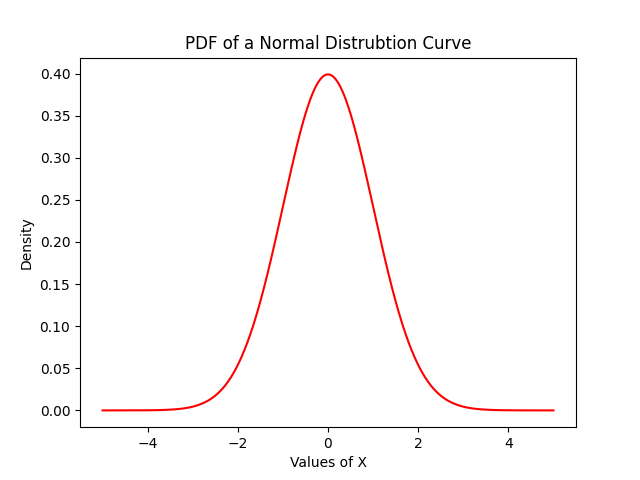
\includegraphics[width=\columnwidth]{C:/GitHub/DataScience/wk_04/plots/PDFNormalDistribution.png}
    \caption{PDF of Normal Distribution Curve} 
\end{figure}

\newpage

\subsection{Creating \& Plotting  Cumulative Distribution Function}
Next, we move on to creating the cumulative distribution function. Using the normalized distribution object, which 
has a passed in mean and standard deviation parameters, and the array of equally spaced numbers using
\texttt{.linspace()}, we then use \texttt{.cdf()} to calculate the cumulative distribution function. \\

We then move to plotting the cumulative distribution function. Using the \texttt{matplotlib} library, we then plot the 
X values that we have generated against the cumulative probabilities that were generated after applying the 
\texttt{.cdf} function. \\

What we ended up getting is the graph as shown below in Figure 2. As we can see, the values range from 0 to 1, 
and we end up getting a cumulative probability that goes from 0 and up to 1, hence producing the curve as shown.
Similar to figure 1, the range of the X values goes from -4 to 4.


\begin{figure}[htbp] 
    \centering
    \noindent
    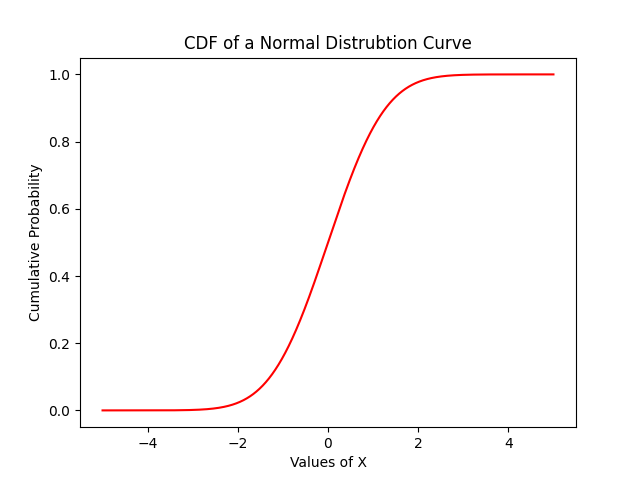
\includegraphics[width=\columnwidth]{C:/GitHub/DataScience/wk_04/plots/CDFNormalDistribution.png}
    \caption{CDF of Normal Distribution Curve} 
\end{figure}

\subsection{The Inverse Cumulative Distribution Function}
Next, we use the inverse cumulative distirbution function in the range of [0,1) and a sample of 1000 times. 
We then move on to plot a histogram of 1000 of these observations.  In order to find the inverse cumulative 
distribution, we use the \texttt{probability point function}, which returns the exact point where the probability of 
everything to the left is equal to the cumulative probability. \\

Lastly, we then move on to plotting the probability point function as a histogram. Using the 
\texttt{matplotlib} library, we then plot the probability value on the x-axis and the cumulative probability on 
the y-axis after applying the \texttt{.ppf}. \\

What we ended up getting is the graph as shown below in Figure 3. Here, the graph gives us the value of the 
random variable at a given cumulative probability. The x-axis represents represents the cumulative probability
and the y-axis represents the frequency of the probabilities. We can obsevse that the graph gives the shape of a
normal distribution curve as a visible peak is seen when the probability is at 0.

\begin{figure}[htbp] 
    \centering
    \noindent
    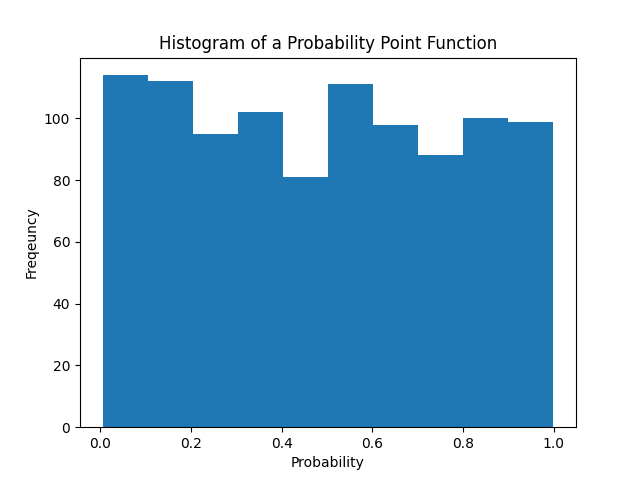
\includegraphics[width=\columnwidth]{C:/GitHub/DataScience/wk_04/plots/PPFHistogram.png}
    \caption{PPF of Normal Distribution Curve} 
\end{figure}

\subsection{Normal Distribution Histogram of 10, 20, 40, 80 and 160 Samples}
Here, we created a function that accepts 2 parameters, a \texttt{scipy} class distribution object and a integer 
\texttt{n}. Here, \texttt{n} is the number of samples to take from the distribution. This method should return a 
list of length n elements, where each element is the value of a single sample. \\

We use the function we created in the cell earlier to generate data and make histograms for each. Here are the 
details of the histograms as shown in the bullet lists and as Figures 4, 5, 6, 7 \& 8 as shown in order.

\begin{itemize}
    \item Normal Distribution of 10 Samples
    \item Normal Distribution of 20 Samples
    \item Normal Distribution of 40 Samples
    \item Normal Distribution of 80 Samples
    \item Normal Distribution of 160 Samples
\end{itemize}

\newpage

\subsubsection{Normal Distribution Histogram of 10 Samples}
When we look at the normal distirbution histogram of 10 samples, we can see that some of the values on the x-axis
don't have any occurences, as clearly displayed when observing the y-axis. Since this occurs at when the values are 
-0.25 and 0.25, we can describe the histogram as multi-modal due to 4 possible peak that occur at =0.75, 0, 0.35 and
at 1. It is quite difficult to deduce the skew of this histogram, as shown below as Figure 4.

\begin{figure}[htbp] 
    \centering
    \noindent
    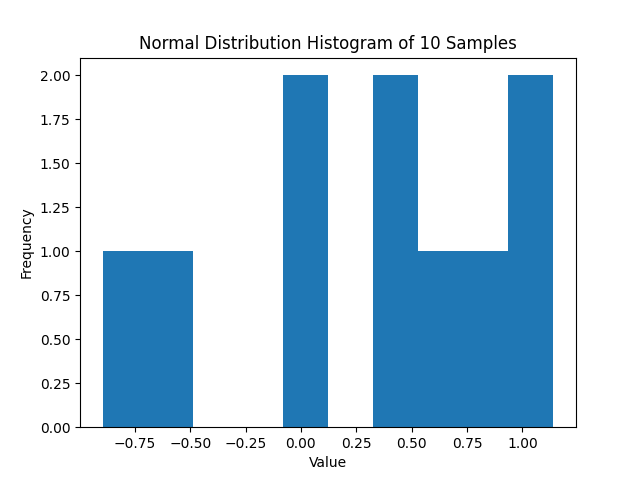
\includegraphics[width=\columnwidth]{C:/GitHub/DataScience/wk_04/plots/NDH of 10 Samples.png}
    \caption{Normal Distribution Histogram of 10 Samples} 
\end{figure}

\subsubsection{Normal Distribution Histogram of 20 Samples}
When we look at the normal distribution histogram of 20 samples, we can see that there are a constant frequency 
between -2 to 2, exluding the downward peak at -1.5 to -1 and 1.5 to 2.0. Due to the upward peak, it can be safe
to deduce that the histogram has a left skew, which is otherwise a negative skew, as shown in Figure 5.

\begin{figure}[htbp] 
    \centering
    \noindent
    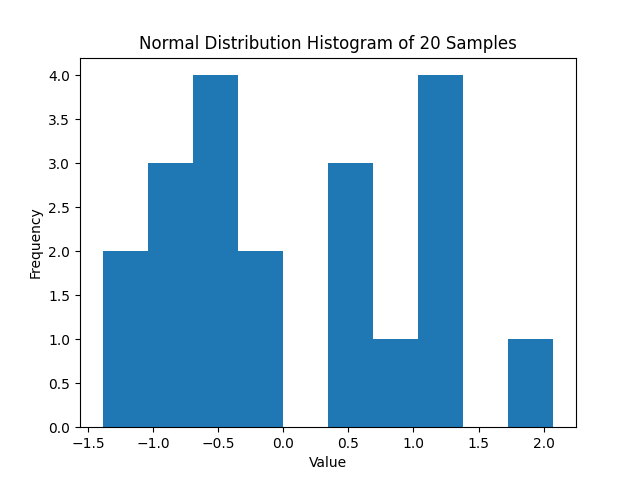
\includegraphics[width=\columnwidth]{C:/GitHub/DataScience/wk_04/plots/NDH of 20 Samples.png}
    \caption{Normal Distribution Histogram of 20 Samples} 
\end{figure}

\subsubsection{Normal Distribution Histogram of 40 Samples}
When we look at the normal distribution histogram of 40 samples, we can see that there is a peak at the center at 
around 0. This peak means that the graph is unimodal and has no skew, as shown in Figure 6.


\begin{figure}[htbp] 
    \centering
    \noindent
    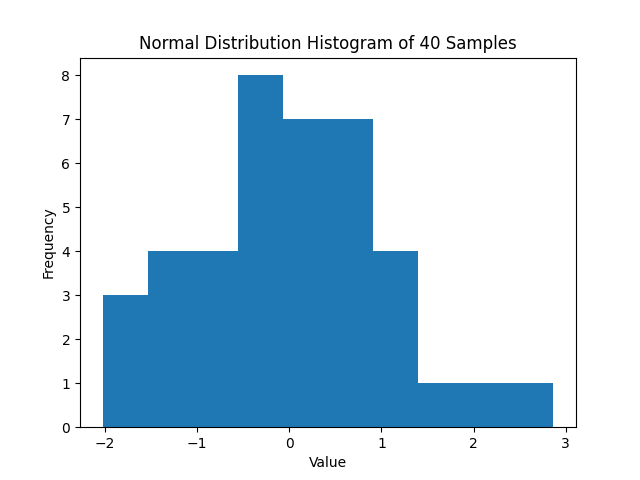
\includegraphics[width=\columnwidth]{C:/GitHub/DataScience/wk_04/plots/NDH of 40 Samples.png}
    \caption{Normal Distribution Histogram of 40 Samples} 
\end{figure}

\subsubsection{Normal Distrubtion Histogram of 80 Samples}
When we look at the normal distribution graph of 80 samples, we can see that there is a peak at -1 on the x-axis.
We can see a second peak that occurs between 0 to 1. As a a result, we can say that the histogram is bimodal. It is 
however, difficult to deduce the skew, as shown in Figure 7. 

\begin{figure}[htbp] 
    \centering
    \noindent
    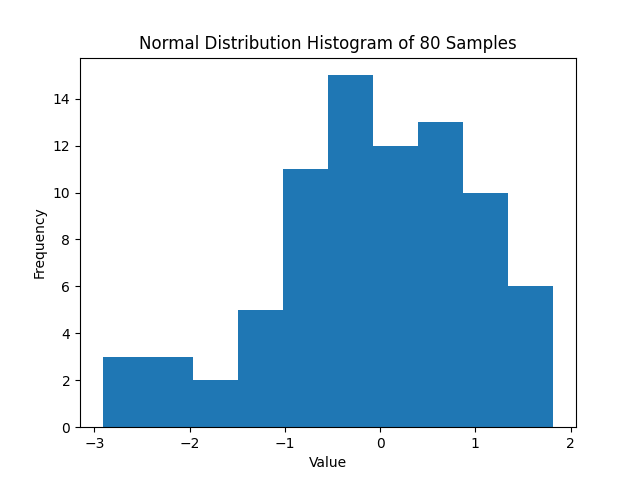
\includegraphics[width=\columnwidth]{C:/GitHub/DataScience/wk_04/plots/NDH of 80 Samples.png}
    \caption{Normal Distribution Histogram of 80 Samples} 
\end{figure}

\newpage

\subsubsection{Normal Distrubtion Histogram of 160 Samples}
When we look at the normal distribution graph of 160 samples, we can see that there is a peak between 0 and 1 on the 
x-axis. As a result, we can deduce that this histogram is unimodal. When we take a look at the positiioning of the
peak, it is observed to be more on the right side, and as result we can say that the histogram is left skewed, 
otherwise known as negatively skewed, as shown in Figure 8.

\begin{figure}[htbp] 
    \centering
    \noindent
    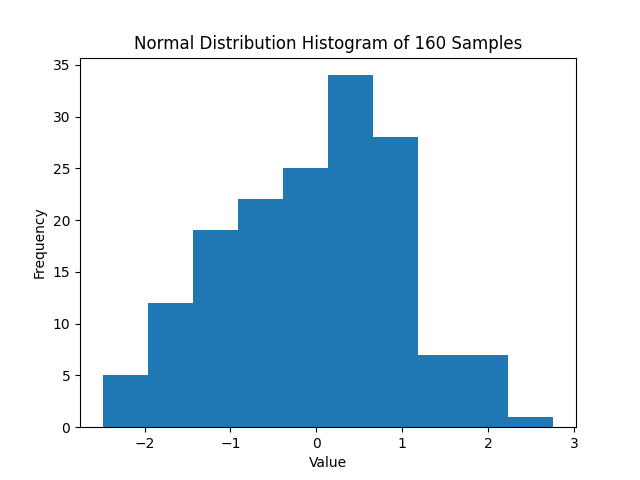
\includegraphics[width=\columnwidth]{C:/GitHub/DataScience/wk_04/plots/NDH of 160 Samples.png}
    \caption{Normal Distribution Histogram of 160 Samples} 
\end{figure}

\subsection{Normal Probability Density Function over Histogram}
For each one of the histograms, as shown in Figures 4 to 8, we directly plot the normal probability density function 
over each of the generated histograms. We achieve this by using the \texttt{seaborn} library. As a result, what we
get is a Probability Density Function line being graphed as shown from Figures 9 to 13. \\

For each of thse figures, we can see that that the line being sketched is designed to fit as best as possible to the
shape of the histogram, and in each of these figures, there is a visible peak that matches the peak of the histogram.
Another common observation of the histograms from Figures 9 to 13 is that the x-axis ranges from around -3 to 3. \\

A notable exception to this is the one in Figure 9, which shows a peak over 0 on the x-axis, although there is no
peak in the histogram.

\begin{figure}[htbp]
    \centering
    \begin{minipage}{0.45\textwidth}
        \centering
        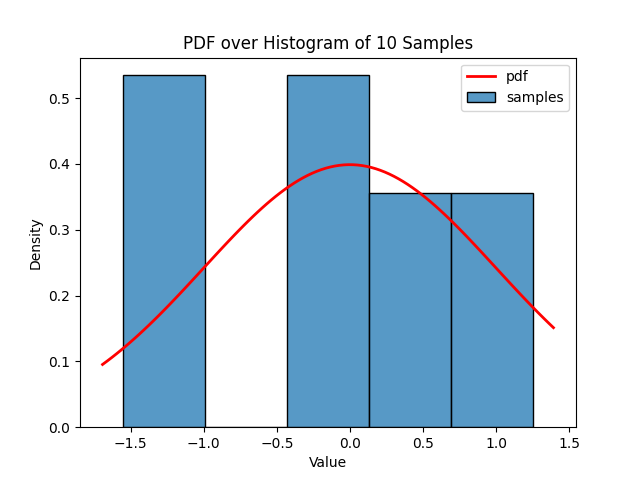
\includegraphics[width=\linewidth]{C:/GitHub/DataScience/wk_04/plots/PDFHistogram 10 Samples.png}
        \caption{Probability Density Function over Histogram of 10 Samples} 
    \end{minipage} \hfill
    \begin{minipage}{0.45\textwidth}
        \centering
        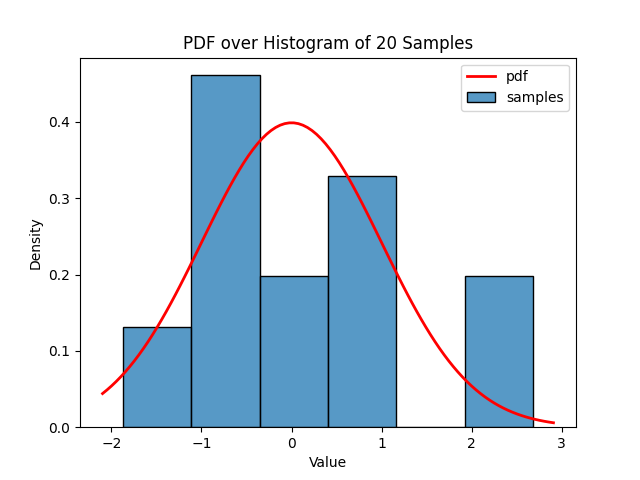
\includegraphics[width=\linewidth]{C:/GitHub/DataScience/wk_04/plots/PDFHistogram 20 Samples.png}
        \caption{Probability Density Function over Histogram of 20 Samples} 
    \end{minipage} 

    \begin{minipage}{0.45\textwidth}
        \centering
        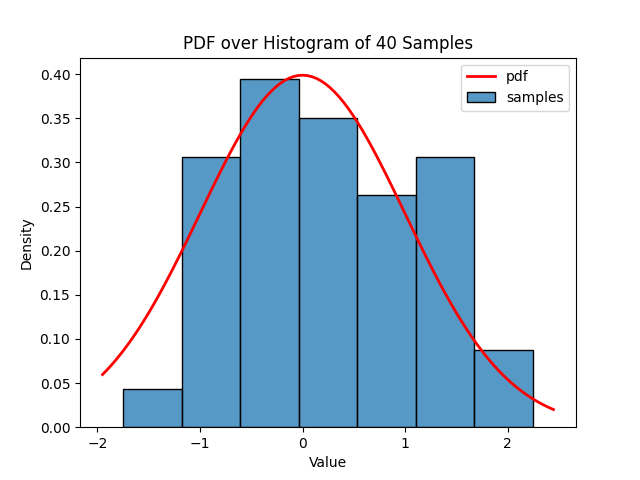
\includegraphics[width=\linewidth]{C:/GitHub/DataScience/wk_04/plots/PDFHistogram 40 Samples.png}
        \caption{Probability Density Function over Histogram of 40 Samples} 
    \end{minipage} 
\end{figure}

\newpage % Page break after 40 samples

\begin{figure}[htbp]
    \centering
    \begin{minipage}{0.45\textwidth}
        \centering
        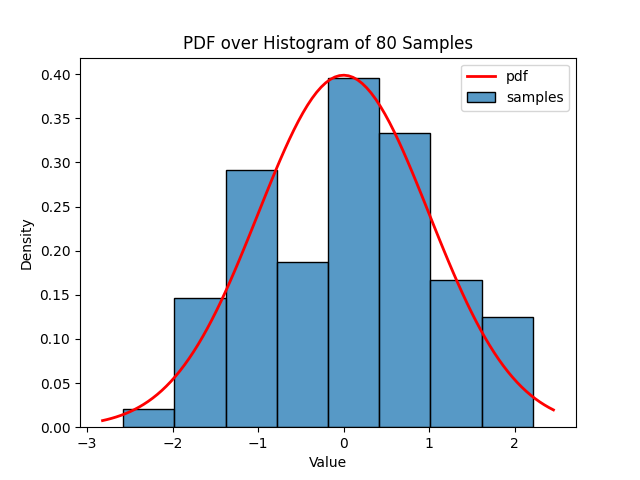
\includegraphics[width=\linewidth]{C:/GitHub/DataScience/wk_04/plots/PDFHistogram 80 Samples.png}
        \caption{Probability Density Function over Histogram of 80 Samples} 
    \end{minipage} 

    \begin{minipage}{0.45\textwidth}
        \centering
        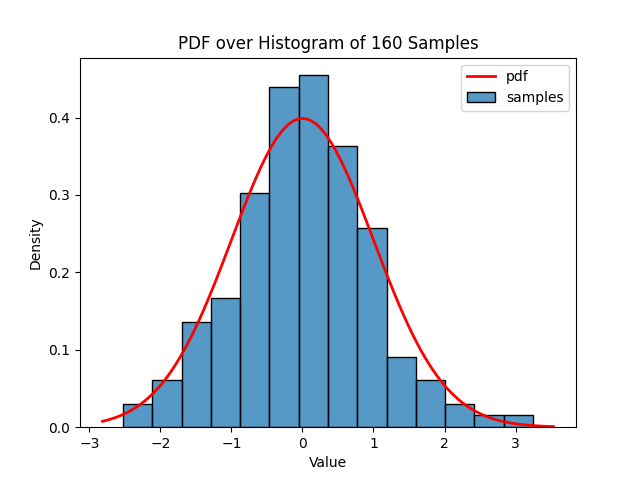
\includegraphics[width=\linewidth]{C:/GitHub/DataScience/wk_04/plots/PDFHistogram 160 Samples.png}
        \caption{Probability Density Function over Histogram of 160 Samples} 
    \end{minipage}
\end{figure}

\subsection{Effect Size vs Iterations}

We start off by drawing two sample groups using the same distribution and the same n, as follows:
\begin{itemize}
    \item the first group should be 25 samples drawn from a normal distribution with mean = 0 and SD = 1
    \item the second group should be 25 different samples drawn from a normal distribution with mean = 0 and SD = 1
\end{itemize}

Next, we calculate the estimated effect size between the two groups. We calculate this by finding the absolute 
value of the difference between group 1 sample mean and group 2 sample mean. \\

We then created a function that accepts two distribution objects, two values of n for number of samples to draw from 
the distributions, and a integer k which is the number of times to loop the sample generations. This method should 
draw from each distribution n times and repeat this process for k iterations. As a result, this method returns 
three lists that are k elements long. The details of the return as follows:

\begin{itemize}
    \item The elements in the first list are the estimated effect sizes at iteration k between the drawn samples of 
    the two distributions
    \item Each element in the second list is a list of the drawn samples from distribution 1 at iteration k
    \item Each element in the third list is a list of the drawn samples from distribtuion 2 at iteration k
\end{itemize}

We then used our defined method to generate two sample groups, each with 25 observations for 1000 iterations. 
We then move to plot a histogram of the effect sizes as shown in Figure 14. \\ 

In this figure, we can see that the highest number of effect sizes range from 0 to $0.25$, as they have the highest
number of iterations. As a result, we get a peak, and the histogram is therefore right-skewed, which is otherwise 
positively skewed.

\begin{figure}[htbp] 
    \centering
    \noindent
    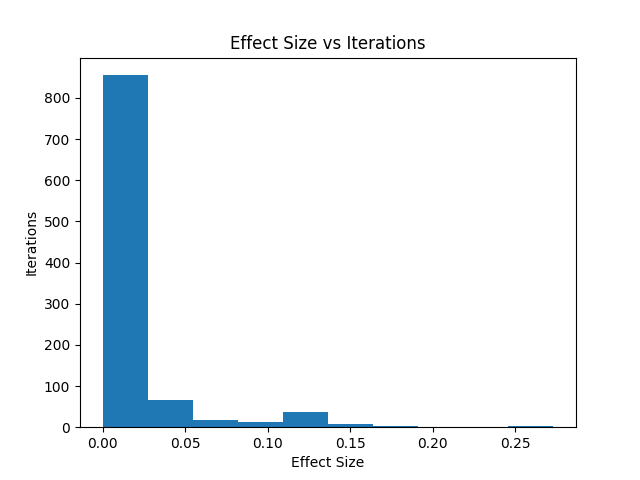
\includegraphics[width=\columnwidth]{C:/GitHub/DataScience/wk_04/plots/EffectSizeIterations.png}
    \caption{Effect Size vs Iterations} 
\end{figure}

\subsection{Histogram of Largest Effect Size of Sample Groups}
Next, we find the index of the largest observed effect size. We use the index to plot the histograms of the
two associated sample groups. As a result, we get Figure 15. \\

When we look at figure 15, we can see the color coded sample one and sampled, depicted as blue and orange. The blue 
singifies the first sample and the orange signifies the second sample. When we look at both of these histograms,
we can deduce the peaks as follows:
\begin{itemize}
    \item For Sample One, there are two peaks at 0 and 1, hence making the histogram bimodal
    \item For Sample Two, there are two peaks at -2 and 0, hence making the histogram bimodal
\end{itemize}

\begin{figure}[htbp] 
    \centering
    \noindent
    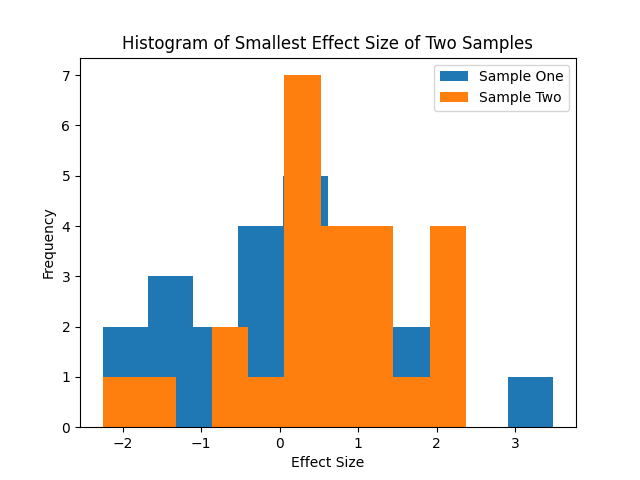
\includegraphics[width=0.5\columnwidth]{C:/GitHub/DataScience/wk_04/plots/HistogramSample.png}
    \caption{Histogram of Largest Effect Size of Two Sample Groups} 
\end{figure}

\newpage

\subsection{Histogram of Effect Size}

Next, we plot the histogram of the estimated effect sizes. We find the index of the minimum effect size and 
plot the two sample groups associated with this index using a histogram, as shown in Figure 16. \\

When we look at this histogram, we can deduce that the histogram is definitely unimodal and has a left skew,
as a result making it negatively skewed. 

\begin{figure}[htbp] 
    \centering
    \noindent
    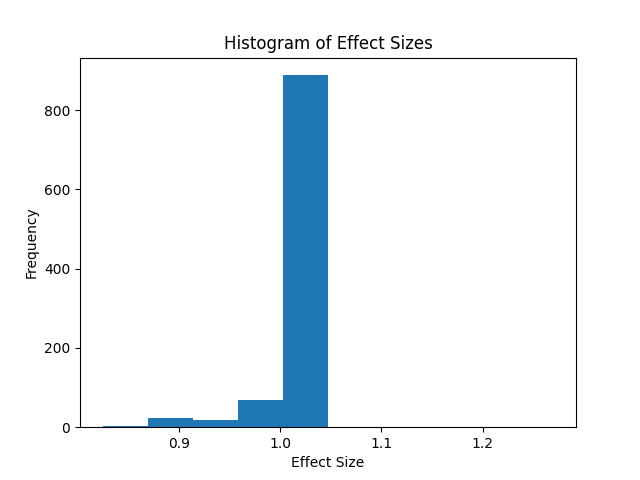
\includegraphics[width=\columnwidth]{C:/GitHub/DataScience/wk_04/plots/HistogramIterations.png}
    \caption{Histogram of Effect Sizes} 
\end{figure}

\subsection{Histogram of Smallest Effect Size of Two Samples }

We started off by instantiating the normal distributions. The first one should have the mean set to 0 and
standard deviation set to 1. The second one should have the mean set to 1 and standard deviation set to 1. 
Next, we run 1000 iterations of sampling 25 values each. \\

This time, the first sample group should consist of 1000 iterations of 25 samples drawn from a normal distribution 
with $\mu = 0$ and $\sigma = 1$, and the second group should consist of 1000 iterations of 25 different samples 
drawn from a normal distribution with $\mu = 1$ and $\sigma = 1$. \\

As a result, we get Figure 17 as shown below. When we look at figure 17, we can see that there are two histograms,
where the blue represents the Sample One and the orange represents the Sample Two. Here are a few observations:
\begin{itemize}
    \item Sample One Histogram: it is a unimodal histogram that has no skew, the peak is at 0.5
    \item Sample Two Histogram: it is a unimodal histogram that has no skew, the peak is at 0.5 but at a Lower
    frequency, hence making it a lower peak. 
\end{itemize}

\begin{figure}[htbp] 
    \centering
    \noindent
    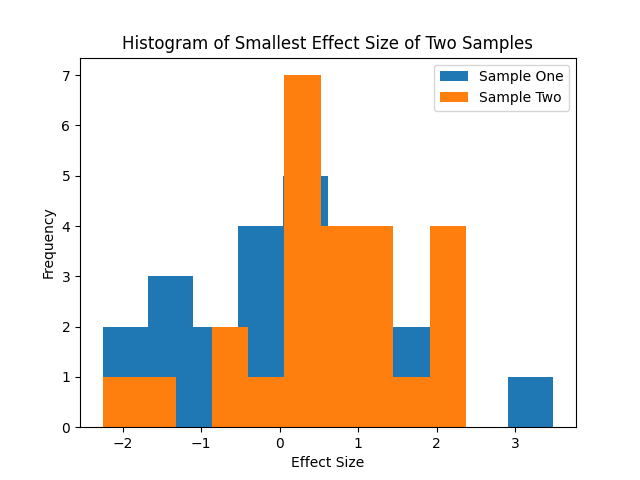
\includegraphics[width=\columnwidth]{C:/GitHub/DataScience/wk_04/plots/HistogramSample.png}
    \caption{Histogram of Smallest Effect Size of Two Samples} 
\end{figure}

\section{Discussion}
We now discuss our findings and conclude everything. We discuss with regards to our tehcniques and some of the
observations that we have deduced with the data we produced and analyzed.

\subsection{Sampling and Normal Distribution}
When we generated our sample values, we found the mean and normal distribution to be approximately zero, 
with a value of \( -4.547 \times 10^{-16} \). With the method we used, we believe that samples generated in this 
manner can approximate the true distribution well. In order to better job of approximating the true distribution,
we can increase the size of the samples, as larger the sample size, the better the sample will approximate the
true distribution. 

\subsection{The Sampling Method}
Moving on, when we began plotting the normal distribution histograms, and as the samples increased from 10 to 160,
we can see that the histograms begin to go from a bi-modal shape to unimodal shape, and as the sample increases from
20 to 160, the peak shifts from the right to the center. 

\subsection{The Type I and II Error}
After we plotted the histograms, we wanted to look at type I and type II errors. They are explained in detail as such:
\begin{itemize}
    \item Type I Error: it is when we reject a null hypothesis when it is true
    \item Type II Error: it when we don't reject the null hypothesis when it is false
\end{itemize}


After establishing an understanding of these errors, we drew two sample groups using the same normal distribution.
The details of the two sample groups are:
\begin{itemize}
    \item Sample Group One has 25 samples drawn from a normal distribution with mean 0 and standard deviation 1
    \item Sample Group Two has 25 different samples drawn from a normal distribution with mean 0 and standard
    deviation 1
\end{itemize}

\newpage

We then calculated the effect size of those two sample groups, and these are the results, respectively:
\begin{itemize}
    \item Mean of Random Sample One:  $0.1057$
    \item Mean of Random Sample Two:  $0.1381$
    \item Estimated Effect Size:  $0.0324$
\end{itemize}

We calculated the effect size by first taking the mean of both random samples. We achieve this by taking the sum of 
all values in both both samples and dividing the length of the number of values in those samples. We then found the 
difference between the mean of both values and took the absolute value of the end result. \\

When we look at these effect sizes in detail, we can find the maximum observed sizes, which appears to be 
$0.27305463084432374$. Interestingly enough, when we graph the histograms of the largest effect size of 
two samples, we can see that the histograms have a bimodal shape. This could mean that for each sample, since there 
are two distinct peaks, the samples may be clustered around two different values. \\

One could deduce that since the bimodal peaks in the histograms appeared in a single trial of a experimental data set
for the maximum observed sizes, this may mean that the data is coming from two different groups. As a result, we can 
conclude that unless there were errors, the two peaks may indicate that there are either two subgroups, or there may 
have been a sampling error. \\

Next, we can look at the minimum observed sizes, which appears to be $0.8241537033428362$. We calculated the expected
effect size in the same way as previously mentioned, where we found the mean of both samples and took the absolute 
value of the difference between them. \\

When we plotted out the histogram of the smallest effect size of the two samples, we see that there is a singular peak,
hence making the histogram unimodal. Furthermore, since the peaks are centered, we can say that there is no skew. As a 
result, this may suggest that most of the data points are around a central value. \\

Given the appearance of the histogram and establishing the fact that the histogram has a single peak, we can conclude 
that there is normal distribution. \\

\subsection{A Journey into Bootstrapping}
Using the dataset from \texttt{data.csv}, we looked into three variables, which have 500 observations. For each of
these variables, we used a for loop of 1,000 iterations to randomly sample the 500 values. We then computed the median
of the resampled data and store the median. \\

After 1,000 iterations, we had 1,000 median values for each variable. We sorted these median values in ascending 
order. Next, we found the 25th value and the 975th value. These values tell us the range within which the true median
is likely to fall 95\% of the time. \\

As a result, we were able to obtain the confidence intervals, and this is how we interpreted it:
\begin{itemize}
    \item Confidence Interval 1: the true value lies between $-1.8950644177598832$ and $1.7796939547361557$ with 
    95\% confidence
    \item Confidence Interval 2: the true value lies between $-1.0887132842610687$ and $2.704221427374523$ with 
    95\% confidence
    \item Confidence Interval 3: the true value lies between $-1.1190463112205178$ and $3.09774608084418$ with 
    95\% confidence
\end{itemize}

When we look at these findings, it means that the true value lies between the stated lower and upper bounds, and we
can declare that with 95\% confidence. \\

Looking further into confidence intervals, there are things we can deduce about the median. Since the confidence
intervals for all three overlap over each other, this may suggest that there is a possibility that the true medians
for the three variables are very similar. 


\end{document}
